\documentclass[10pt]{beamer}
\usepackage[utf8]{inputenc}
\usetheme{default}
\usecolortheme{dove}
\usepackage{textpos}
\usepackage{tikz}
\usepackage{grid-system}

\usepackage[T1]{fontenc}
\usepackage[sfdefault]{AlegreyaSans}
\renewcommand*\oldstylenums[1]{{\AlegreyaSansOsF #1}}

\AtBeginSection[]
{
  \begin{frame}<beamer>
    \frametitle{Übersicht}
    \tableofcontents[currentsection]
  \end{frame}
}

\usebackgroundtemplate%
{%
    \tikz[overlay,remember picture]
    \node[opacity=0.26, at=(current page.south east),anchor=south east,inner sep=0pt] {
        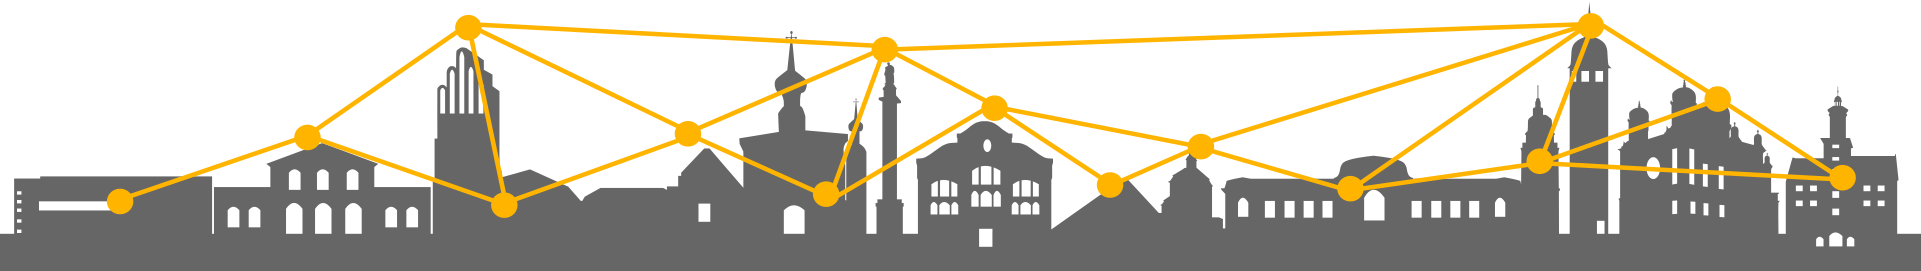
\includegraphics[width=\paperwidth]{images/footer_dark}
    };
}

  \addtobeamertemplate{frametitle}{}{
    \begin{textblock*}{0cm}(\textwidth-0.85cm,-0.85cm)
      \begin{figure}[h]
        \def\svgwidth{1.5cm}
        \input{logo.pdf_tex}
      \end{figure}
    \end{textblock*}
  }

\title{Freifunk Darmstadt}
\author{}
\institute[Inst.]{eine Initiative des Chaos Darmstadt e.V.}
\date{\footnotesize 23. Mai 2016}

\begin{document}

{
  \usebackgroundtemplate{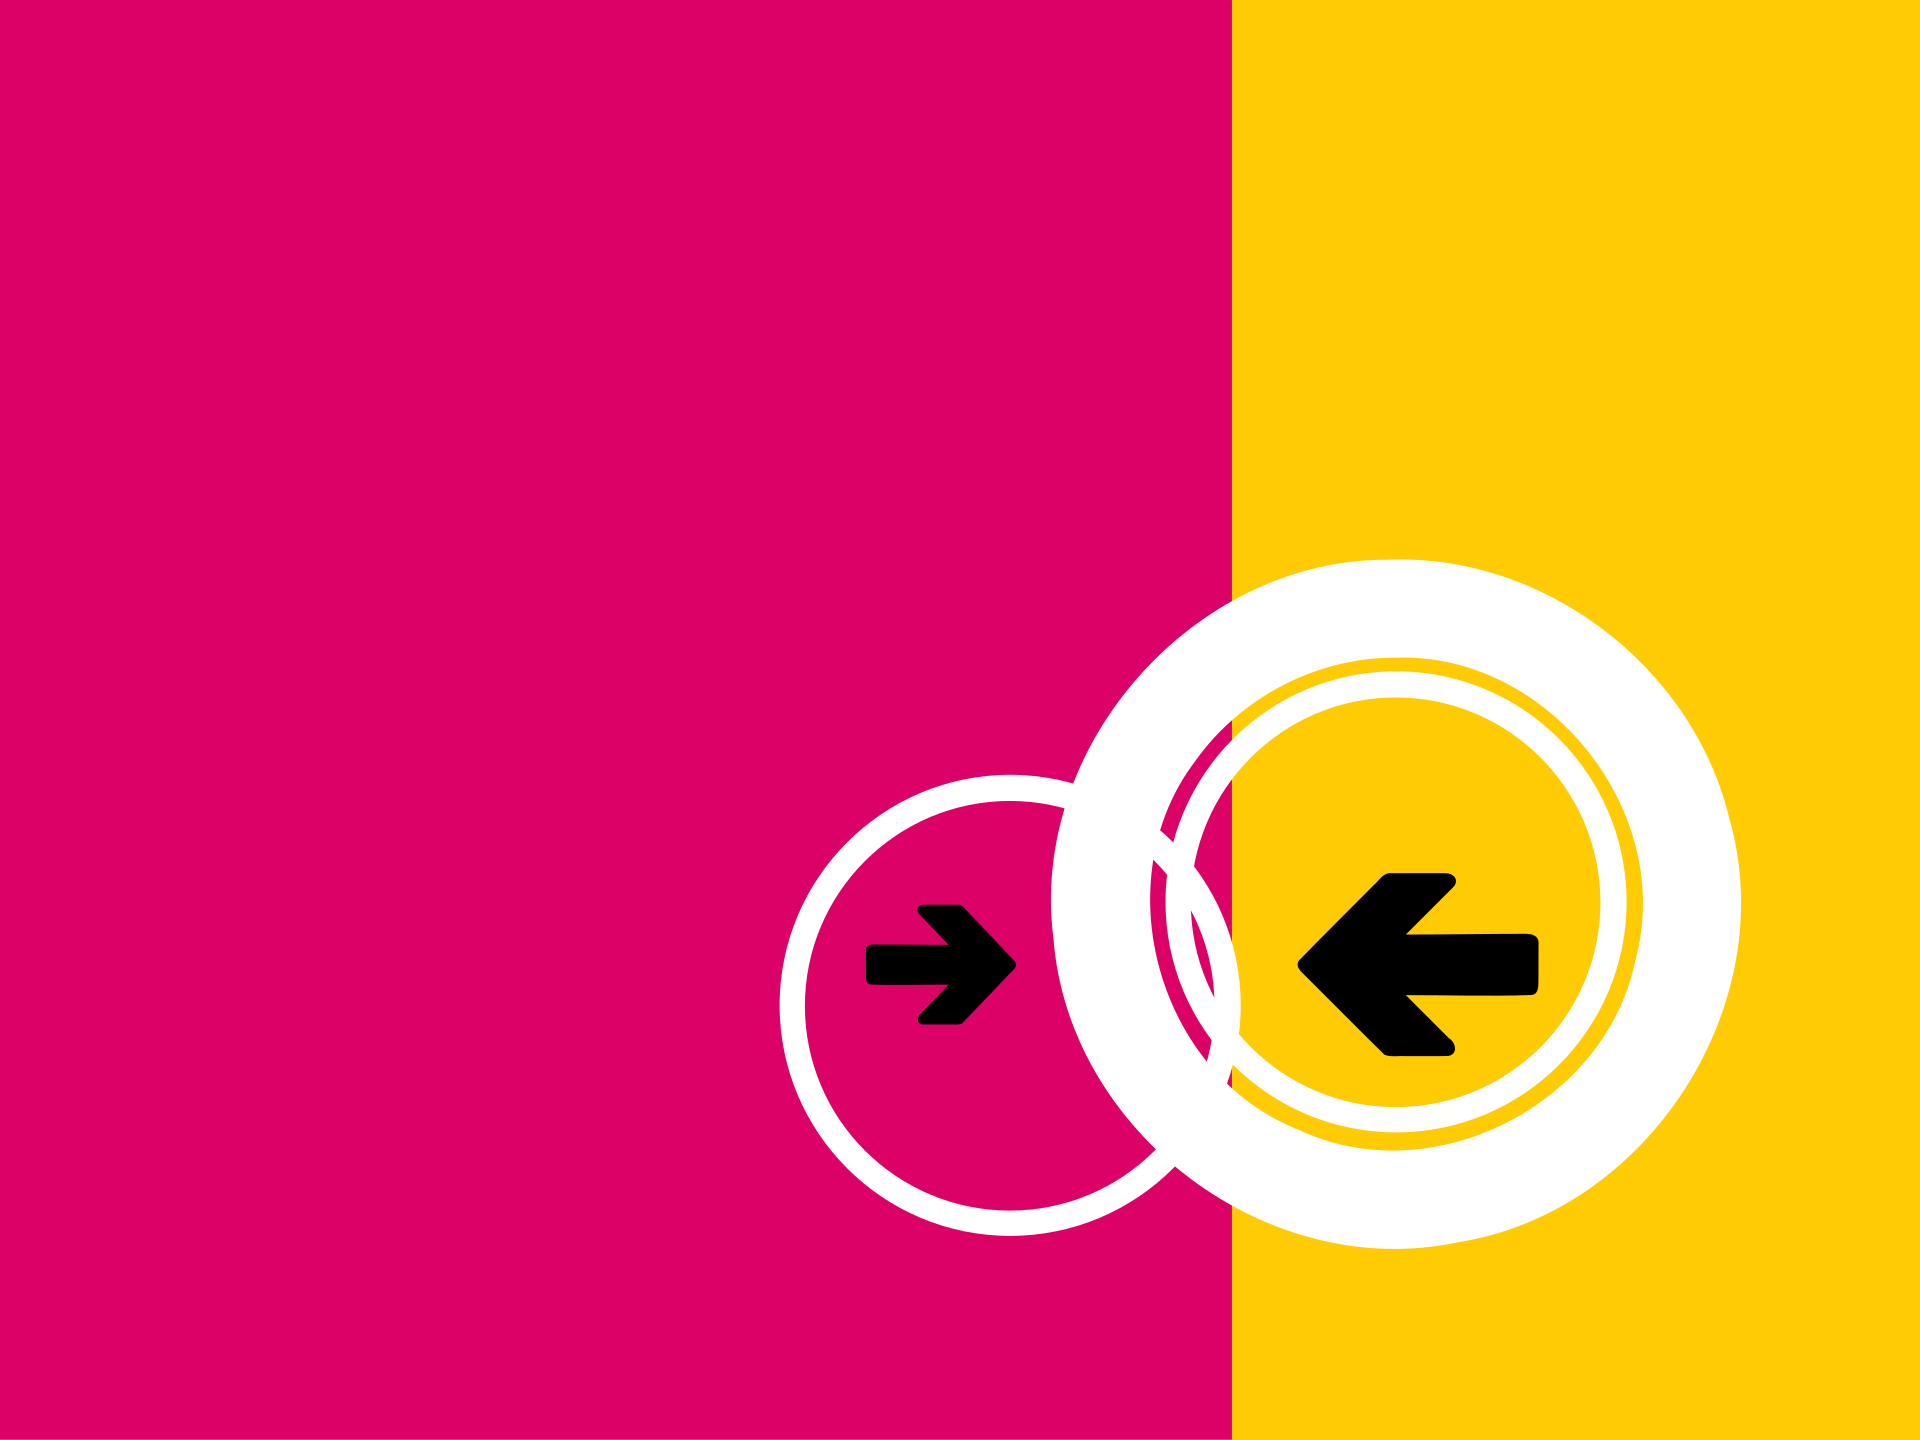
\includegraphics[width=\paperwidth]{images/logo_magenta_yellow.png}}
  \begin{frame}
    \begin{huge}
      Freifunk Darmstadt
    \end{huge}
    \vspace{0.25em}
    \newline
    Dein freies WLAN-Netz
    \newline
    \vspace{0.5em}
    \newline
    \small{23. Mai 2016}
    \vfill
  \end{frame}
}
  \begin{frame}{Übersicht}
    \tableofcontents
  \end{frame}

  \section{Wer wir sind}

  \begin{frame}{Freifunk Darmstadt: Das wichtigste auf einen Blick}
    \begin{center}
    \begin{itemize}
	  \item Teil einer bundes- und weltweiten Bewegung für offene Netze
	  \item Initiative des Chaos Darmstadt e.\,V.
	  \item nicht kommerziell
	  \item Erstes Treffen im Februar 2014
      \item 15 Freifunker im Kernteam
    \end{itemize}
    \vfill
    
\includegraphics[width=.3\textheight]{images/cda}
    \end{center}
  \end{frame}


  \section{Was ist Freifunk}

  \begin{frame}{Was ist Freifunk?}
      \begin{center}
        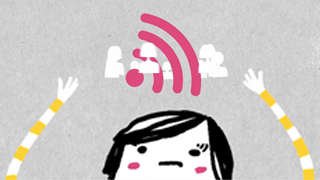
\includegraphics[width=3.6cm]{images/up}
      \end{center}
      Wie wäre es, wenn\ldots
      \begin{itemize}
        \pause
        \item online jeder mit jedem kommunizieren könnte\pause, \textit{\textbf{ohne eine Firma}, bei der man sich anmelden muss?}
        \pause
        \item wir unsere eigenen Dienste betreiben könnten\pause,  \textit{\textbf{ohne} auf einen \textbf{zentralen kommerziellen Anbieter} angewiesen zu sein?}
        \pause
        \item Kommunikation jederzeit möglich ist\pause, \textit{auch wenn unsere herkömmliche \textbf{Infrastruktur ausfällt}}
      \end{itemize}
    \end{frame}

    \begin{frame}{Und wie sieht das in der Praxis aus?}
      \begin{center}
        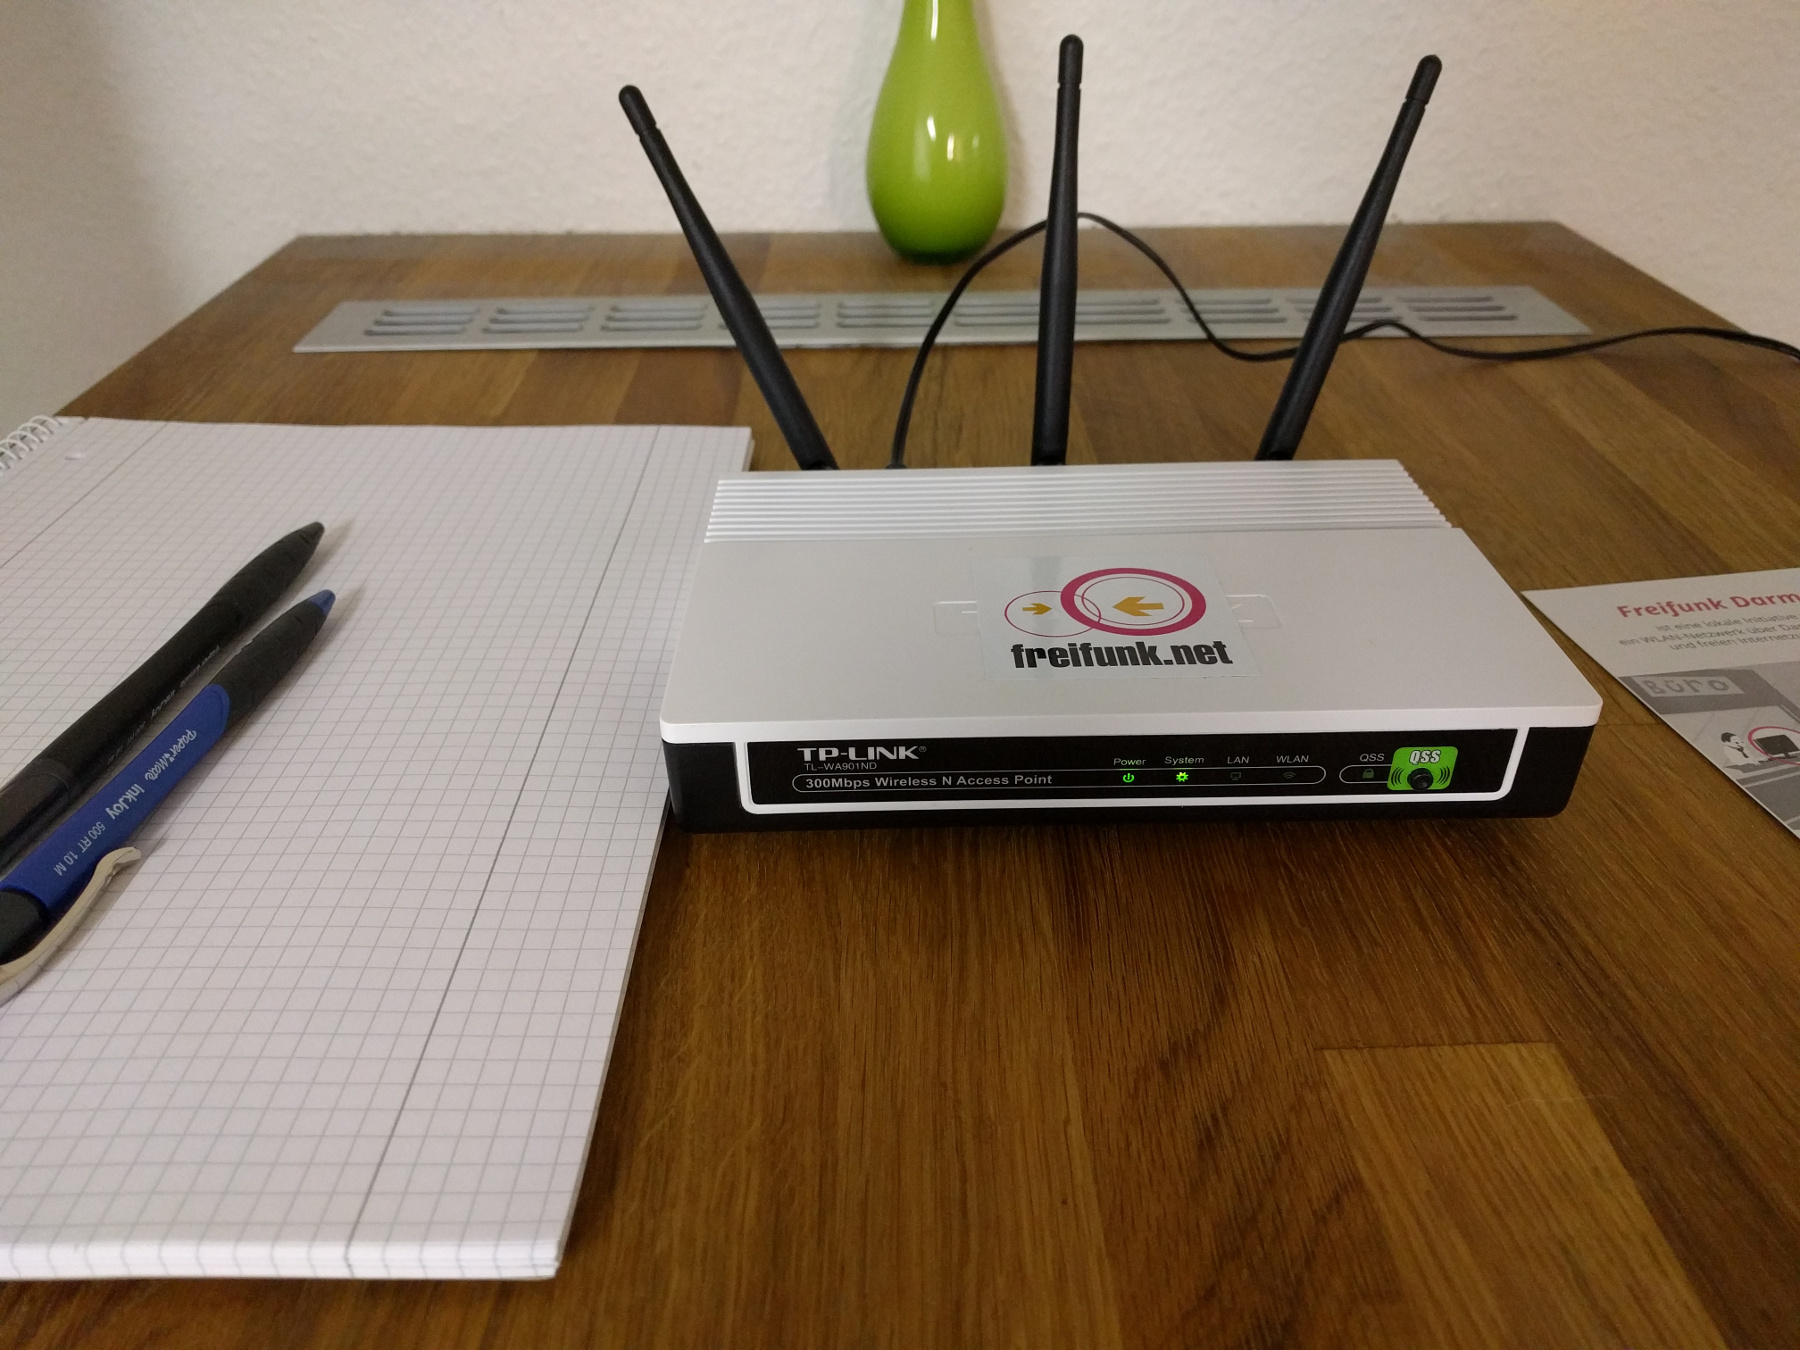
\includegraphics[width=7cm]{images/homerouter}
      \end{center}
    \end{frame}

    \begin{frame}{Und wie sieht das in der Praxis aus?}
      \begin{center}
        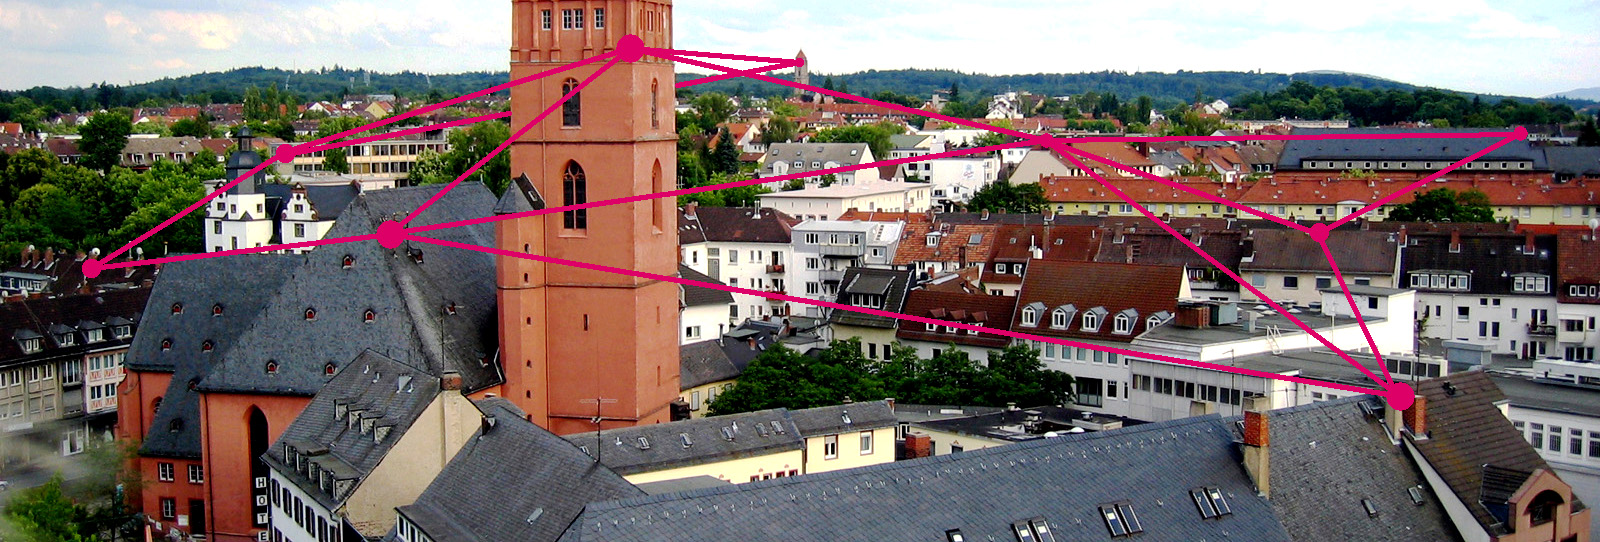
\includegraphics[width=10cm]{images/banner-stadtkirche-darmstadt}
      \end{center}
    \end{frame}

    \begin{frame}{Warum ein freies Netz?}

      \begin{center}
        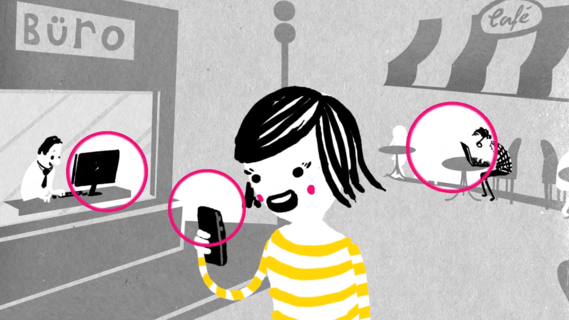
\includegraphics[width=4.5cm]{images/verbindet}
      \end{center}

      \begin{itemize}
        \item \emph{gleichberechtigt} Netzwerkdienste anbieten und nutzen
        \begin{itemize}
          \item Telefonieren und Chatten (z.B. Tox, Ricochet, Mumble)
          \item dezentrales Social-Media (z.B Diaspora, Twister)
          \item lizenzfreies Community-Radio (In Aufbau, hilf uns dabei!)
          \item deine Idee!
        \end{itemize}
        \item Internetzugänge \emph{teilen}
        \item \emph{krisensichere} Netzwerktopologie
      \end{itemize}
      \vfill
    \end{frame}

  \begin{frame}{Ziele von Freifunk}
    \begin{columns}[T]
     \begin{column}{5cm}
        \begin{itemize}
          \item \textbf{Verständnis von Kommunikationsnetzen} sowie deren Auswirkungen auf die Gesellschaft fördern
          \item Teilnahme der Bevölkerung an \textbf{Forschung und Aufbau} dezentraler Netze
          \item \textbf{Wissen und Software} öffentlich zugänglich machen
          \item Beteiligung an politischen Prozessen, um \textbf{rechtliche Voraussetzungen} für freie Netze zu schaffen
        \end{itemize}
      \end{column}
      \begin{column}{5cm}
        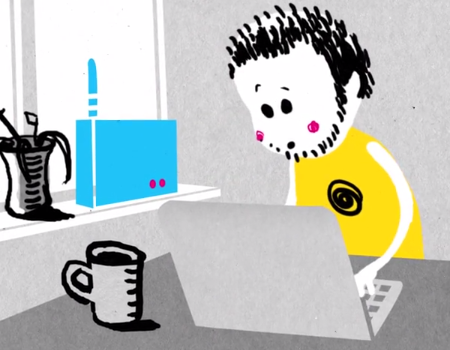
\includegraphics[width=0.9\textwidth]{images/install}
      \end{column}
    \end{columns}
  \end{frame}

    \begin{frame}{Freifunk: offen und öffentlich}
    \begin{columns}[c]
      \begin{column}{5cm}
        
\includegraphics[width=\textwidth]{images/open}
        \newline \tiny \url{https://flickr.com/photos/29355306@N06/15613972489}
      \end{column}
      \begin{column}{7cm}
        \begin{itemize}
          \item \textbf{gemeinschaftlicher} Aufbau und Betrieb des Netzes $\Rightarrow$ Mitmachnetz
          \item anonymer, \textbf{unzensierter Zugang} zu Netz und Diensten
          \item \textbf{keine Unterscheidung} nach Ort oder Geldbeutel
          \item \textbf{Datensparsamkeit}
        \end{itemize}
      \end{column}
    \end{columns}
  \end{frame}

  \begin{frame}{Dezentral aufgebaut und organisiert}
      \large \textbf{Deutschlandweite Initiative für \emph{freie} Netze.}
      \begin{center}
        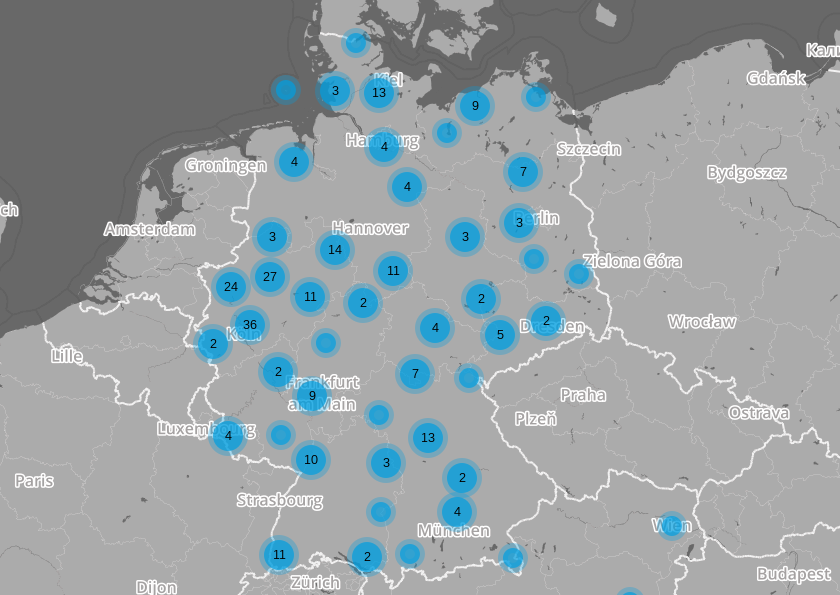
\includegraphics[height=9em]{images/2016-02-17_map-de}
      \end{center}
      \begin{itemize}
        \item fast 300 lokale Gruppen
        \item über 33.000 offene Zugangspunkte\footnote{\url{https://freifunk.net/wie-mache-ich-mit/community-finden/}}
      \end{itemize}
    \end{frame}

  \section{Wie Freifunk funktioniert}

  \begin{frame}{Ohne Freifunk}
    \begin{center}
      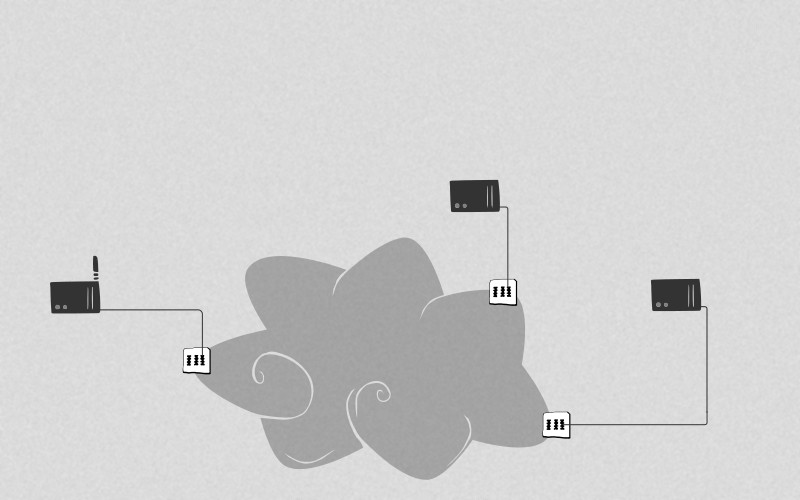
\includegraphics[height=5cm]{images/network_1}\\
      \vspace{1em}
      Geschlossene WLAN-Netze, welche nicht miteinander kommunizieren
      \vspace{1em}
    \end{center}
  \end{frame}

  \begin{frame}{Mit Freifunk}
    \begin{center}
      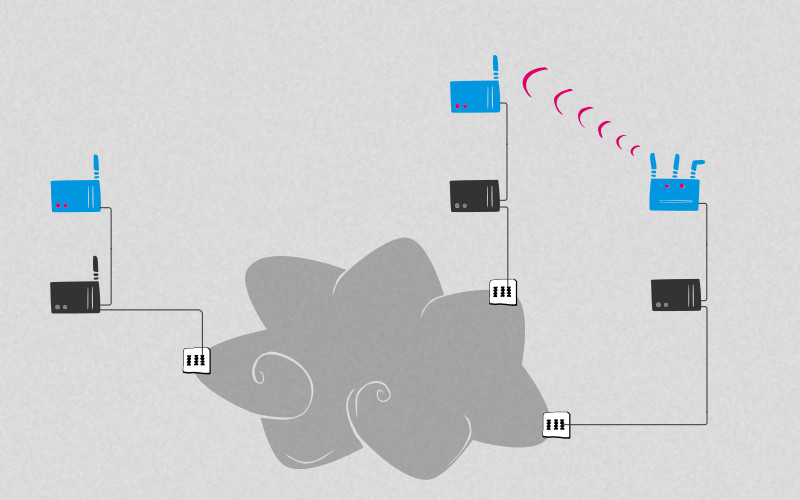
\includegraphics[height=5cm]{images/network_2}\\
      \vspace{1em}
      Freifunk-Knoten spannen ein freies Netz auf
      \vspace{1em}
    \end{center}
  \end{frame}

  \begin{frame}{Verminderung der digitalen Kluft}
    \begin{center}
      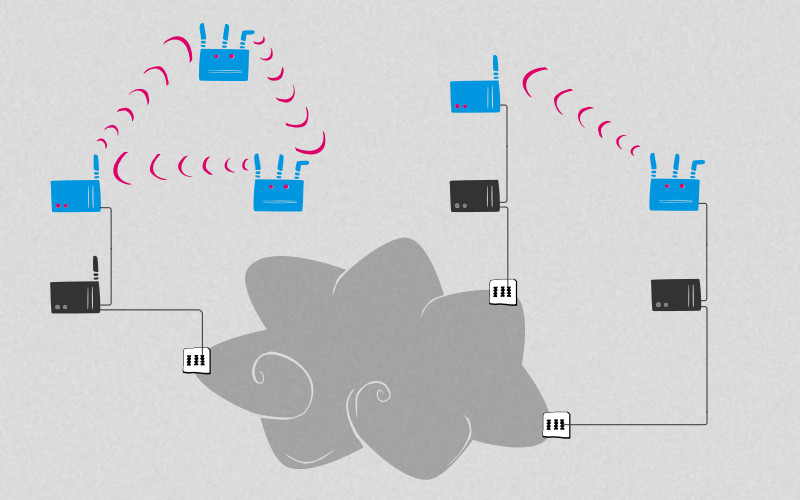
\includegraphics[height=5cm]{images/network_3}\\
      \vspace{1em}
      Neue Knoten ohne Internetzugang kommen hinzu
      \vspace{1em}
    \end{center}
  \end{frame}

  \begin{frame}{Das Heimnetz bleibt privat}
    \begin{center}
      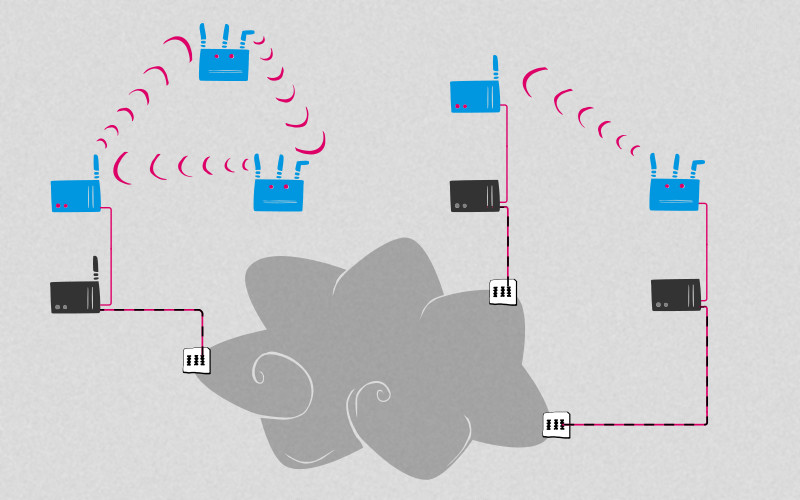
\includegraphics[height=5cm]{images/network_4}\\
      \vspace{1em}
      Eigenes Heimnetz und Freifunk-Netz bleiben getrennt
      \vspace{1em}
    \end{center}
  \end{frame}

  \begin{frame}{Zugang zum Internet}
    \begin{center}
      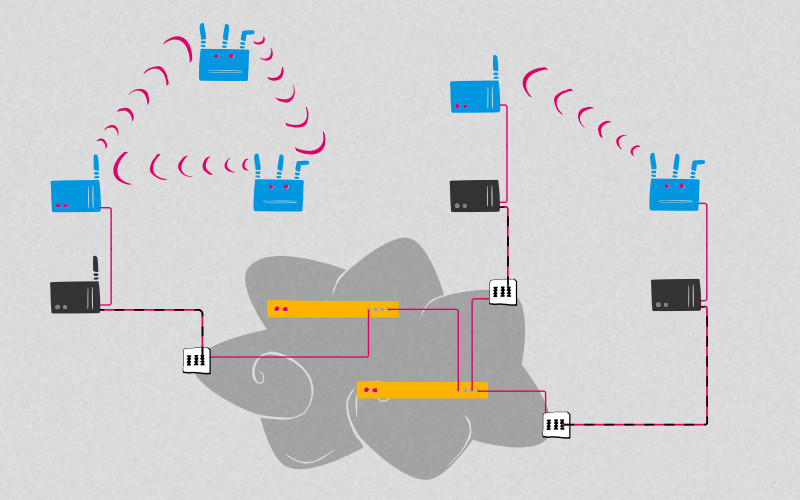
\includegraphics[height=5cm]{images/network_5}\\
      \vspace{1em}
      Gateways stellen Internetzugang bereit
      \vspace{1em}
    \end{center}
  \end{frame}

  \begin{frame}{Wie ein solches Netzwerk aussieht}
    \begin{center}
      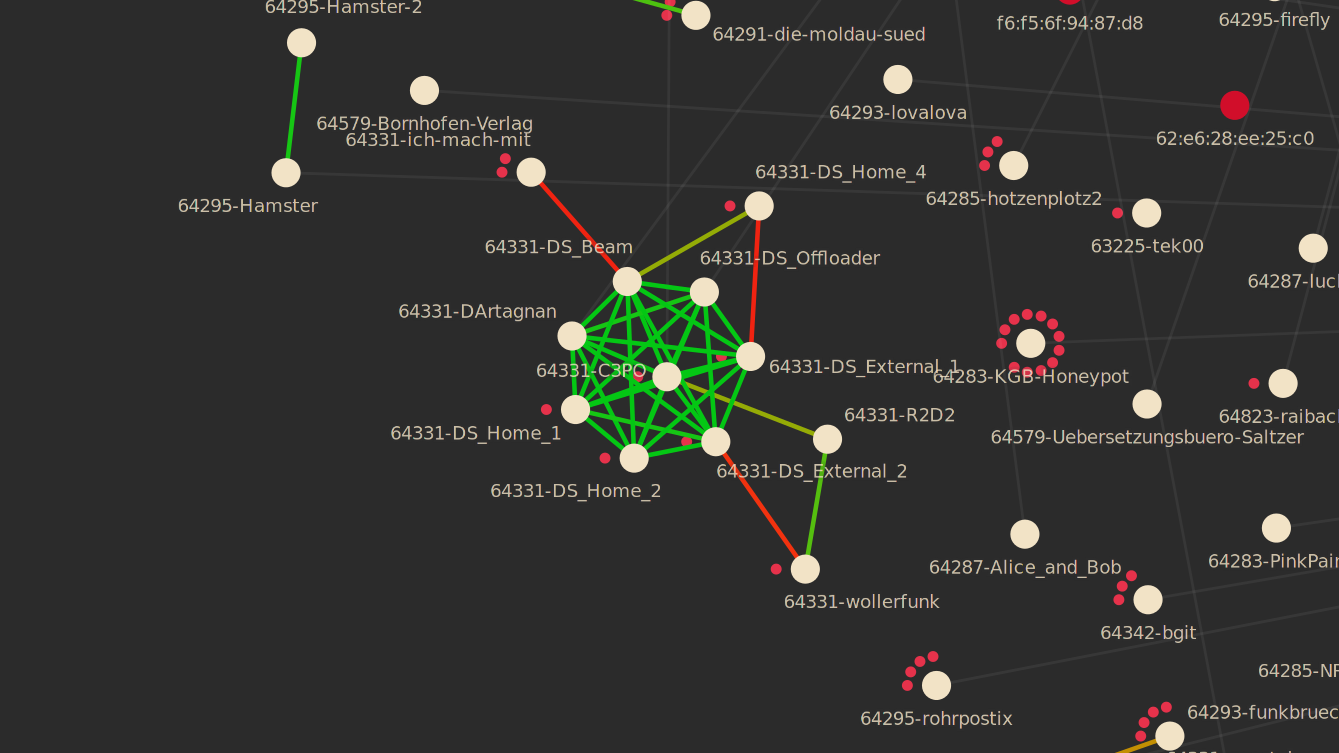
\includegraphics[height=5cm]{images/mesh_small}\\
      \vspace{1em}
      Magenta Punkte stehen für aktuell verbundene Nutzer
      \vspace{1em}
    \end{center}
  \end{frame}

  \begin{frame}{Wie ein solches Netzwerk aussieht}
    \begin{center}
      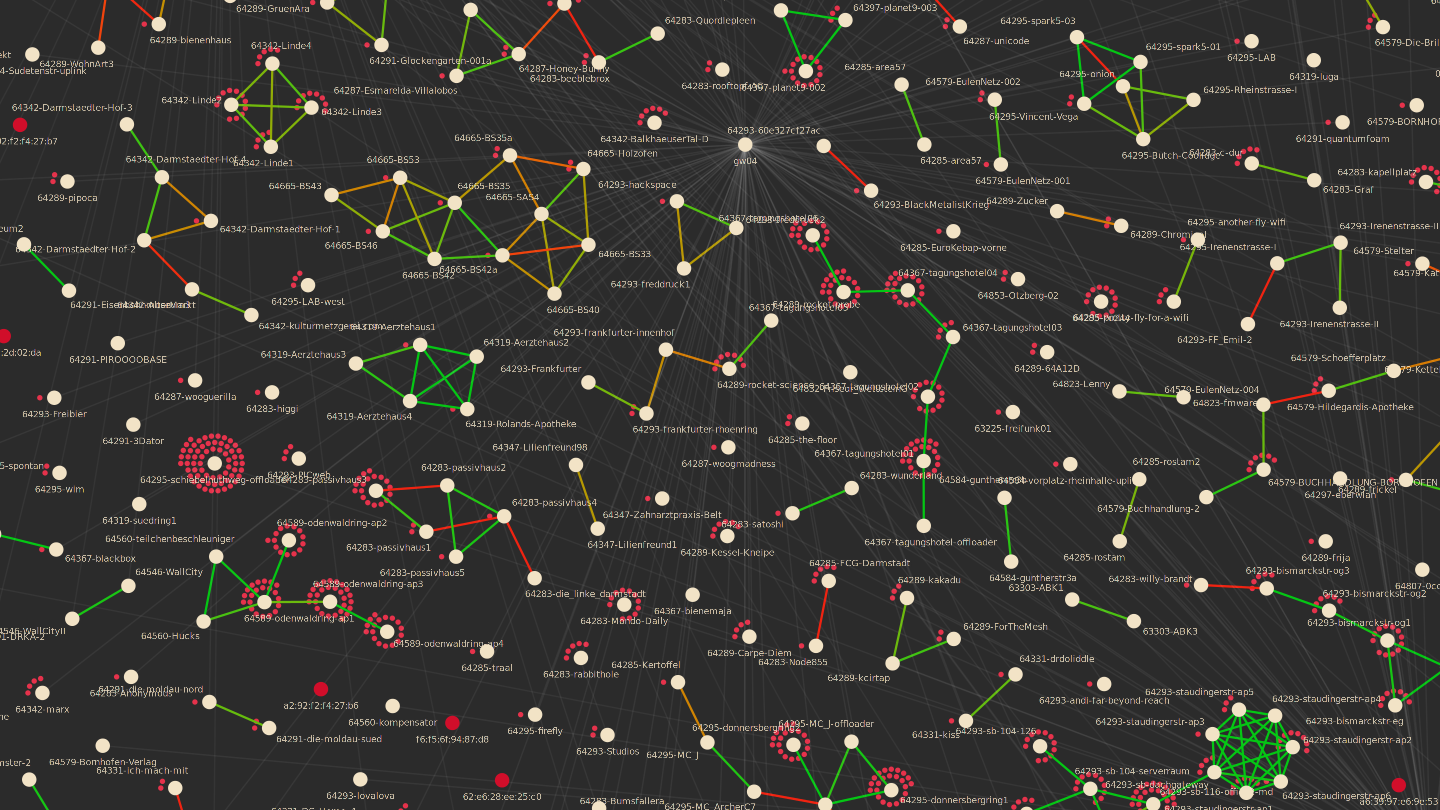
\includegraphics[height=5cm]{images/mesh_medium}\\
      \vspace{1em}
      Farbige Linien stellen Verbindungen zwischen den Knoten dar
      \vspace{1em}
    \end{center}
  \end{frame}

  \section{Freifunk in Darmstadt}

  \begin{frame}{Freifunk Darmstadt - Mai 2016}
    \begin{center}
      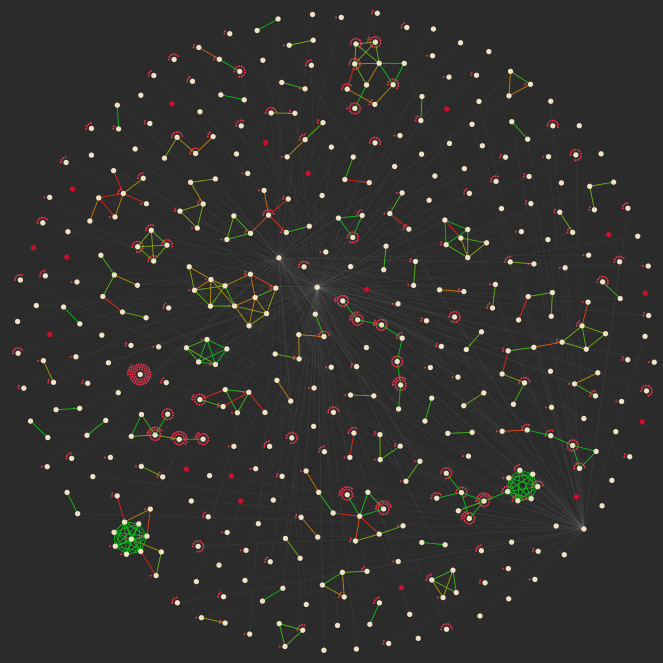
\includegraphics[height=6cm]{images/mesh_big}\\
    \end{center}
  \end{frame}

  \begin{frame}{Freifunk Darmstadt - Mai 2016}
    \begin{center}
      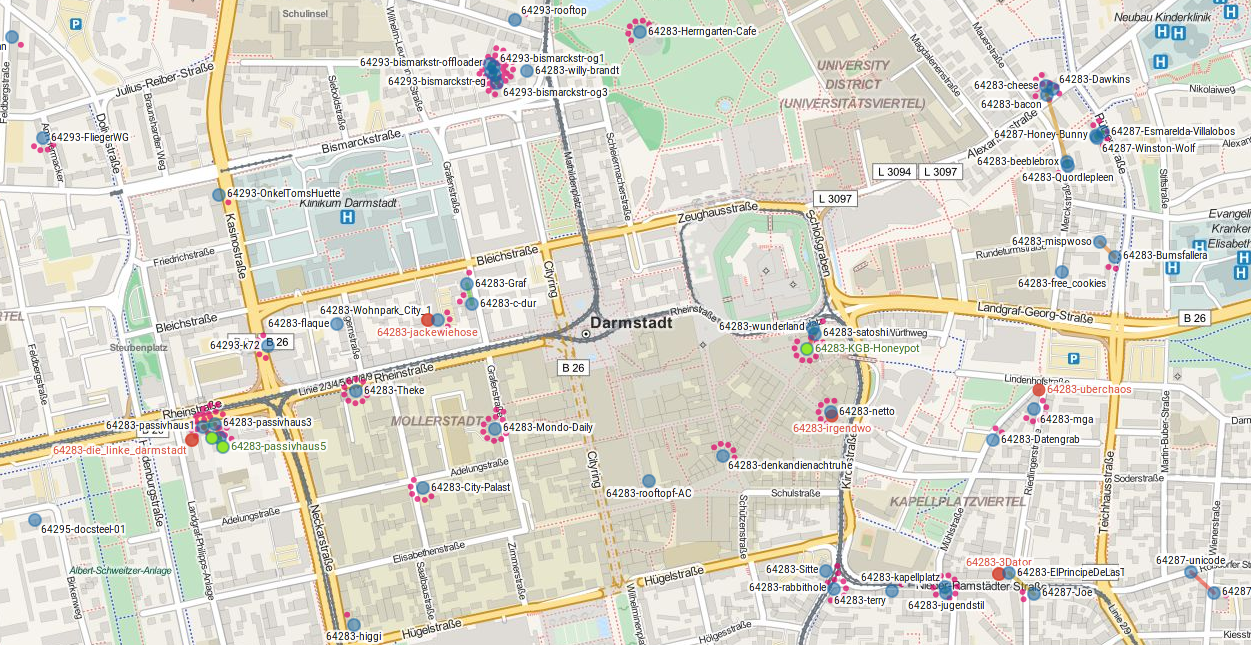
\includegraphics[height=5.5cm]{images/2016-05_map-innenstadt}\\
    \end{center}
  \end{frame}

  \begin{frame}{Freifunk Darmstadt - Mai 2016}
    \begin{center}
      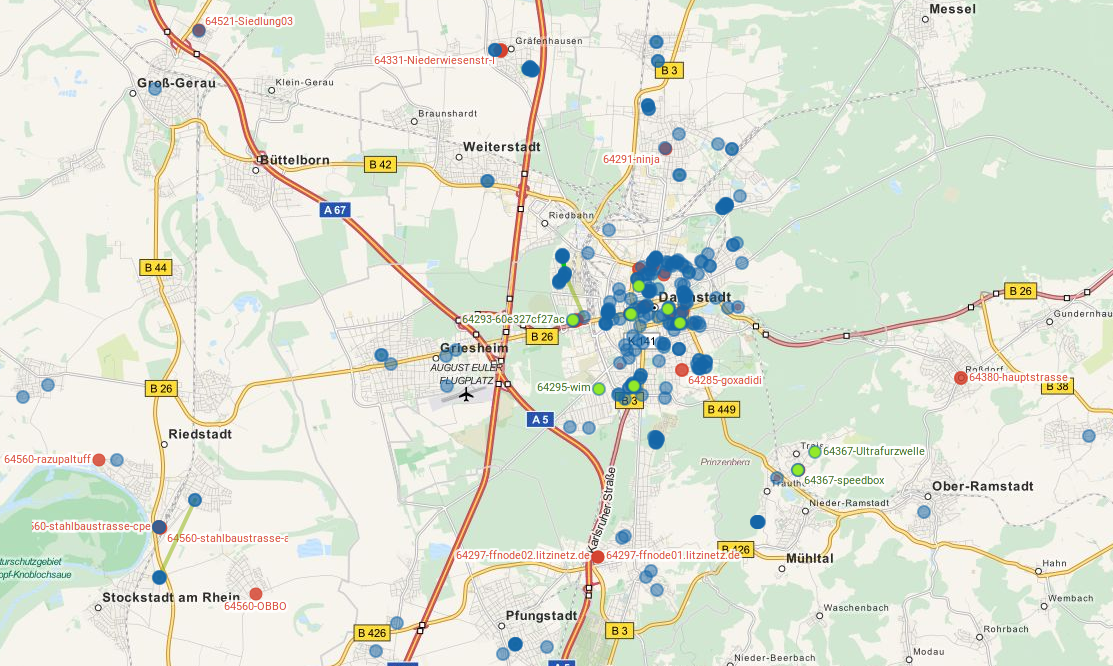
\includegraphics[height=5.5cm]{images/2016-05_map-umland}\\
    \end{center}
  \end{frame}

  \begin{frame}{Freifunk Darmstadt: In Zahlen}
    \begin{itemize}
	  \item ungefähr 1000 gleichzeitige Nutzer täglich
	  \item \emph{über} 400 Freifunk-Knoten in Darmstadt und Umland
	  \item ca. 80 TB an Internetverkehr \emph{jeden Monat}
    \end{itemize}
    \begin{center}
      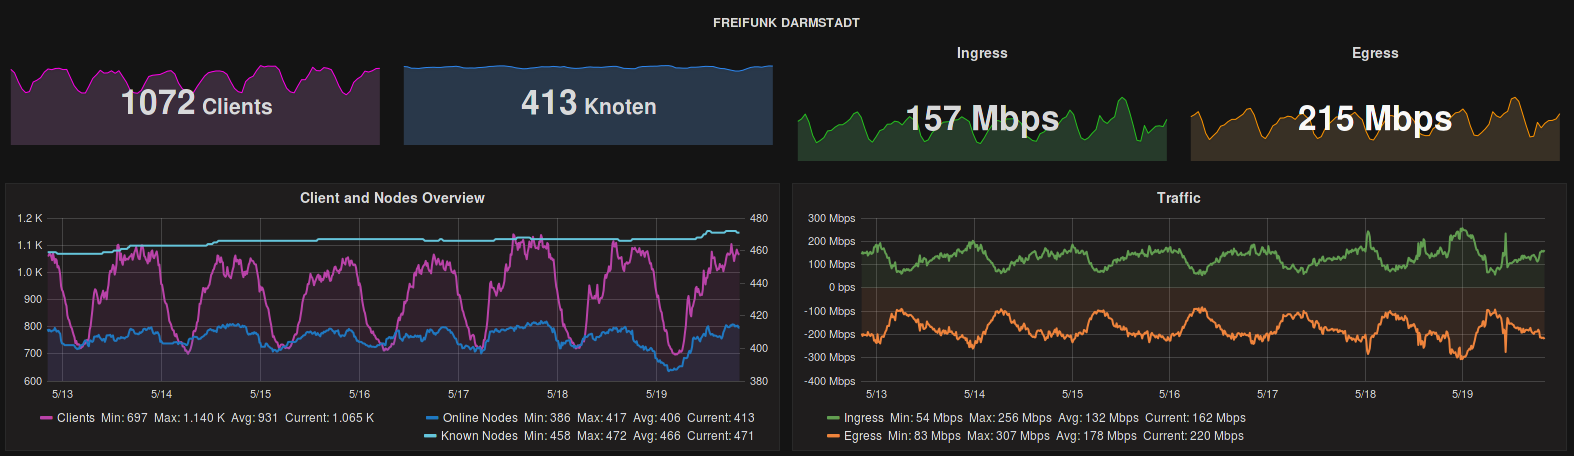
\includegraphics[height=3cm]{images/2016-05_grafana}
    \end{center}
  \end{frame}

  \begin{frame}{Aktuelle Aufgaben}
    \begin{columns}[T]
      \begin{column}{5cm}
        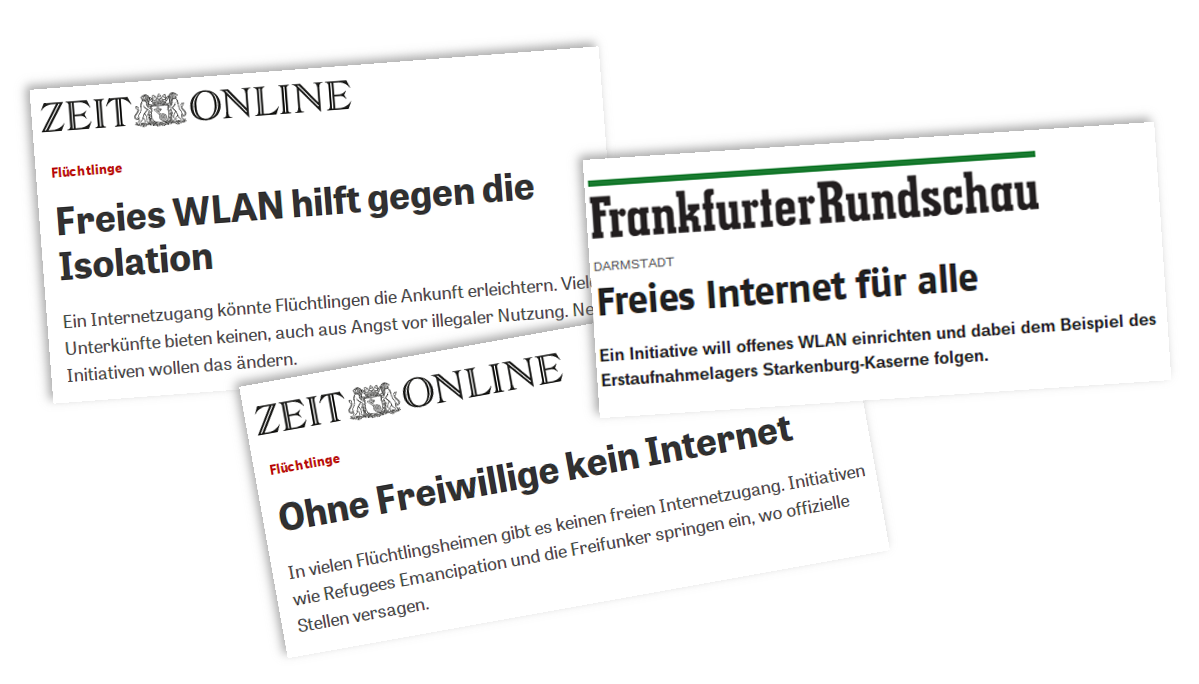
\includegraphics[width=\textwidth]{images/2015-10_presse-fluechtlinge}
        \vspace{1em}
        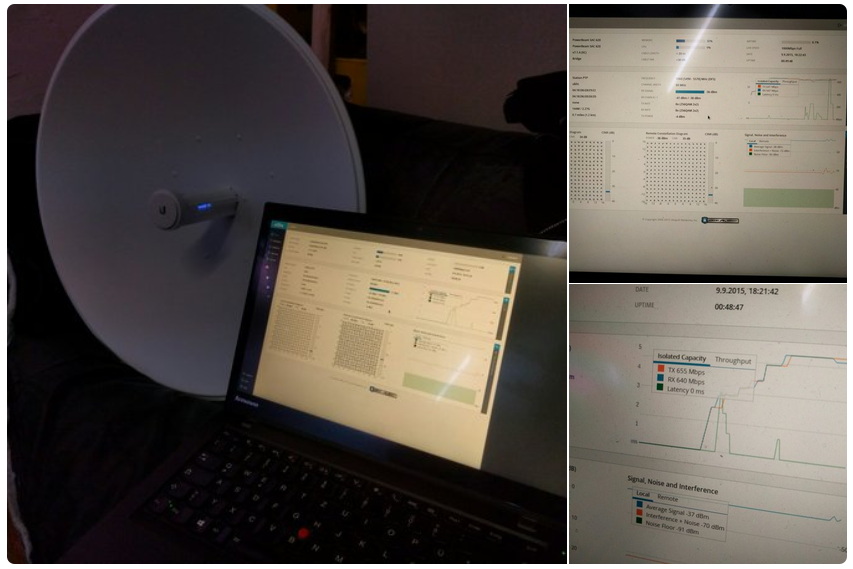
\includegraphics[width=\textwidth]{images/powerbeam-mit-laptop}
      \end{column}
      \begin{column}{7cm}
      \begin{itemize}
        \item \large Flüchtlingsunterkünfte mit Internet versorgen\\
        \tiny in ua. Darmstadt, Mühltal, Stockstadt, Modautal\\
        \end{itemize}
        \begin{itemize}
          \item Freifunk-Software weiterentwickeln
          \item Unterstützer gewinnen
          \item Öffentliche Plätze versorgen
          \item Verbindungen zu anderen Communities aufbauen
          \item Wireless-Backbone über Darmstadt
        \end{itemize}
        \end{column}
      \end{columns}
    \end{frame}

  \begin{frame}{Wir freuen uns auf Euch!}
    \hspace{1em}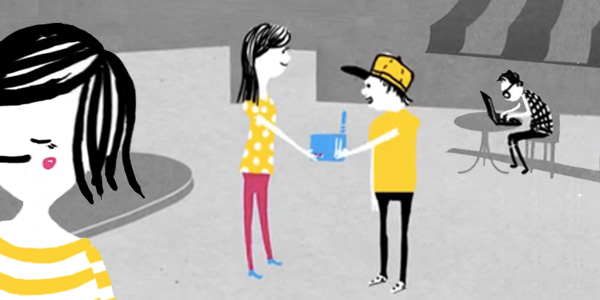
\includegraphics[width=0.6\textwidth]{images/router}
    \begin{itemize}
      \item wir treffen uns jeden Montag um 18:30 Uhr
      \item außerdem online im Chat (\url{https://chat.darmstadt.freifunk.net/})
      \item Twitter \texttt{@FreifunkDA}
      \item weitere Kontaktmöglichkeiten auf unserer Webseite:\\
      \url{https://darmstadt.freifunk.net/kontakt/}
    \end{itemize}
  \end{frame}

\end{document}
